\chapter{Extending \sofa}\label{chapter:es}

This chapter presents how different types of classes can be added to \sofa{} to implement new behaviors.

\section{Adding a new DynamicObject}

A DynamicObject is responsible for implementing the behavior of a given type of body. It contains the degrees of freedoms (\textit{DOFs}) of the body (within the MechanicalObject class), as well as its mass (i.e. how the body moves given an applied force).

To add a new DynamicObject in \sofa, the following steps are required:

\begin{enumerate}
\item Specify the type of its DOFs in a \textcode{DataTypes} class.
\item Create the \textcode{DynamicObject} derived class implementing the behaviors of the body, or instantiate an existing class with you \textit{DataTypes} class if already available.
\item Create a method to create an instance of the body given an XML node.
\item Register the new DynamicObject in the \textcode{Sofa::Components::XML::DynamicNode::Factory} factory.
\item Create a XML scene file containing a DynamicModel with the \textit{type} of our class.
\item Have fun!
\end{enumerate}

If the new class will only be created procedurally, then only the first two steps are required.

We will now detail these steps using the example of an object containing a set of one-dimensional particles.

The code corresponding to this example is available in the following files:
\begin{description}
\item[Sofa/doc/src\_examples/example3/MassObject1d.h]~\\
 Declaration of MassObject1d.
\item[Sofa/doc/src\_examples/example3/MassObject1d.cpp]~\\
 Creation from XML and registration in the Factory
\item[Sofa/doc/src\_examples/example3/Main.cpp]~\\
 Main program
\item[Sofa/doc/src\_examples/example3/test1.scn]~\\
 Test scene file
\end{description}

\subsection{Specification of the Degrees of Freedom}\label{sec:DOF}

The data types used by the body are specified in a class containing the following definitions:

\begin{description}
\item[Coord]~\\
 Type of DOFs.
\item[Deriv]~\\
 Type of derivatives (velocity, forces, displacements).
\item[VecCoord]~\\
 Container of DOFs.
\item[VecDeriv]~\\
 Container of derivatives.
\item[void set(Coord\& c, double x, double y, double z)]~\\
 Utility method to set the value of a point.
\item[void add(Coord\& c, double x, double y, double z)]~\\
 Utility method to add a value to a point (for applyTranslation).

\end{description}

In our example, we can use double as the type of DOFs and std::vector as containers:

\begin{code_cpp}
class Vec1dTypes
{
public:
  typedef double Coord;
  typedef double Deriv;
  typedef std::vector<Coord> VecCoord;
  typedef std::vector<Deriv> VecDeriv;
  
  /// Here we only use the first coordinate
  static void set(Coord& c, double x, double /*y*/, double /*z*/)
  {
    c = x;
  }
  
  static void add(Coord& c, double x, double /*y*/, double /*z*/)
  {
    c += x;
  }
};
\end{code_cpp}

\subsection{Body Behaviors Implementation}

In \sofa{} a DynamicObject does not implement the time integration algorithm, which is handled by an separate Solver. Instead, it implements basic operations, such as compute forces, combine several vectors, etc. Of these operations, most are only dependant on the types of DOFs, or are computed through external classes (ForceFields for instance). Only 3 operations related to the mass remain to be implemented by DynamicObject subclasses:

\begin{description}
\item[computeForce] must be modified to add gravity ( $\ve f = \ve f + \ma M \ve g$ ).
\item[accFromF] must be implemented to convert forces to accelerations ( $\ve a = \ma M^{-1} \ve f$ ).
\item[addMDx] must be implemented to multiply a given displacement by the mass ( $ \ve r = \ve r + \ma M \ve dx$ ).
\end{description}

In our example, a class \textcode{MassObject} already exists to handle object represented as a set of particles. So we just need to instantiate it to the type of DOFs we want to use:

\begin{code_cpp}
typedef MassObject<Vec1dTypes> MassObject1d;
\end{code_cpp}

As a reference, here is how MassObject implements the 3 operations mentioned earlier:

\begin{code_cpp}
template <class DataTypes>
void MassObject<DataTypes>::addMDx(VecDeriv* res, VecDeriv* dx)
{
  for( unsigned i=0; i<dx->size(); ++i )
    (*res)[i] += (*dx)[i] * masses[i].mass;
}


template <class DataTypes>
void MassObject<DataTypes>::accFromF(VecDeriv* a, VecDeriv* f)
{
  a->resize(f->size());
  for( unsigned i=0; i<f->size(); ++i )
    (*a)[i] = (*f)[i] / masses[i].mass;
}


template <class DataTypes>
void MassObject<DataTypes>::computeForce(VecDeriv* result)
{
  Inherit::computeForce(result);
  // Add Gravity
  for (unsigned int i=0;i<result->size();i++)
  {
    (*result)[i]+=gravity*masses[i].mass;
  }
}
\end{code_cpp}

\subsection{Instantiation from XML}

\sofa{} implements a mechanism to load a scene from a XML file using a two step process:

\begin{enumerate}
\item The XML file is parsed and converted to a tree of Node class.
\item Each node use a Factory to instantiate the described object.
\end{enumerate}

A DynamicObject is described by a \textcode{Sofa::Components::XML::DynamicNode}. It contains the type of the class to instantiate, as well as a set of string attributes. To build our DynamicObject from this description we need a function to construct and configure a new instance given the pointer to the XML::DynamicNode. This can either be a constructor in our class, or an external function with the following prototype:
\begin{code_cpp}
namespace Sofa { namespace Components { namespace Common {
void create(MyDynamicObject*& obj, XML::Node<Sofa::Abstract::DynamicModel>* arg);
} } }
\end{code_cpp}
where \textcode{MyDynamicObject} is the name of our new class.

\textbf{Note:} the inclusion in the \textcode{Sofa::Components::Common} namespace is necessary for the Factory class to find our function. If anyone find a better design removing this requirement please tell me!

Typically, the object will either be constructed from attributes given in the XML node, or using an external description file.

Our 1D particles example is simple enough not to require an external file. We can implement a creation function as follow:

\begin{code_cpp}
/// Read a vector of scalars from a string.
void readVec1(std::vector<double>& vec, const char* str)
{
  vec.clear();
  if (str==NULL) return;
  const char* str2 = NULL;
  for(;;)
  {
    double v = strtod(str,(char**)&str2);
    std::cout << v << std::endl;
    if (str2==str) break;
    str = str2;
    vec.push_back(v);
  }
}

namespace Sofa { namespace Components { namespace Common {
/// Construct a MassObject1d object from a XML node.
void create(MassObject1d*& obj, XML::Node<Sofa::Abstract::DynamicModel>* arg)
{
        obj = new MassObject1d();
  obj->clear();
  std::vector<double> mass;
  std::vector<double> pos;
  std::vector<double> vel;
  std::vector<double> fixed;
  readVec1(mass,arg->getAttribute("mass"));
  readVec1(pos,arg->getAttribute("position"));
  readVec1(vel,arg->getAttribute("velocity"));
  readVec1(fixed,arg->getAttribute("fixed"));
  if (arg->getAttribute("gravity"))
  {
    obj->setGravity(atof(arg->getAttribute("gravity")));
  }
  unsigned int maxsize = mass.size();
  if (pos.size()>maxsize) maxsize = pos.size();
  if (vel.size()>maxsize) maxsize = vel.size();
  double defaultmass = (mass.empty()?1.0:*mass.rbegin());
  while (mass.size()<maxsize)
    mass.push_back(defaultmass);
  double defaultpos = 0;
  if (!pos.empty()) defaultpos = *pos.rbegin();
  while (pos.size()<maxsize)
    pos.push_back(defaultpos);
  double defaultvel = 0;
  if (!vel.empty()) defaultvel = *vel.rbegin();
  while (vel.size()<maxsize)
    vel.push_back(defaultvel);
  for (unsigned int i=0;i<maxsize;i++)
  {
    obj->addMass(pos[i], vel[i], mass[i], 0.0,
      (std::find(fixed.begin(), fixed.end(), (double)i)!=fixed.end()));
  }
} } } }
\end{code_cpp}

Note that this function is quite long, as it construct vectors of values (masses, positions, velocities) from strings. For simpler cases, where only a filename is required for instance, generic creation functions are provided:
\begin{code_cpp}
namespace Sofa { namespace Components { namespace Common {
/// Construct a MassObject1d object from a XML node using an external file.
void create(MassObject1d*& obj, XML::Node<Sofa::Abstract::DynamicModel>* arg)
{
  XML::createFromFilename(obj, arg);
} } } }
\end{code_cpp}
However it is then necessary to implement the external file loading method.

\subsection{Factory Registration}

Once all functionalities are implemented, it is necessary to register the new class in the \textcode{Sofa::Components::XML::DynamicNode::Factory} factory in order for \sofa{} to know about it. This requires adding the following "magic" line:

\begin{code_cpp}
Creator< XML::DynamicNode::Factory, MassObject<Vec1dTypes> >
  MassObject1dClass("MassObject1d");
\end{code_cpp}

This command will register our class to the Factory during the initialization of the program. For this to work we must still ensure our code is linked in the final binary. To do this we must add the following line in the .cpp file containing the Creator command:
\begin{code_cpp}
SOFA_DECL_CLASS(MassObject1d)
\end{code_cpp}
and then add a corresponding line in a .cpp file used during the execution of the program (such as the file containing the main() function, or in Sofa/Components/init.cpp if the new class is integrated in \sofa{}):
\begin{code_cpp}
SOFA_INIT_CLASS(MassObject1d)
\end{code_cpp}
This last step is required to work around portability issues, and might be removed if a better solution is found.

When the given type name is used in an XML file, the Factory will now be able to construct our custom DynamicObject.

\subsection{Testing}

Our new class can now be loaded by writing a small XML file:

\begin{code_xml}
<Scene dt="0.005" showBehaviorModels="1" showCollisionModels="1" showMappings="1" showForceFields="1">
	<Group>
		<Solver type="RungeKutta4"/>
		<DynamicModel type="MassObject1d" name="M1" position="0 1 2 3 4 5" fixed="5" gravity="-9.8"/>
	</Group>
</Scene>
\end{code_xml}

To run it, go to \textcode{Sofa/doc/src\_examples/example3} and execute
\begin{code_bash}
./run test1.scn
\end{code_bash}

\begin{figure}
\centering
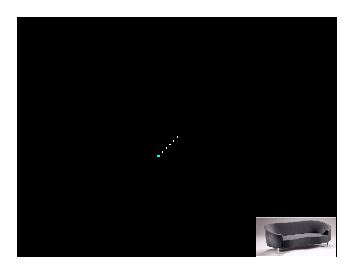
\includegraphics[width=0.5\linewidth]{fig/mass1d}
\caption{Test scene with 6 1D particles.}
\end{figure}

\section{Adding a new Mapping}

Many existing objects in \sofa{} expect to work with 3D particles. To be able to use them with our 1D particles, we can create a MechanicalMapping which will convert information between the two representations.

Adding a new Mapping in \sofa{} requires the following steps:

\begin{enumerate}
\item Create the \textit{Mapping} or \textit{MechanicalMapping} derived class computing the mapping from the input model to the output, and accumulating forces back for MechanicalMappings.
\item Create a method to create an instance of the mapping given an XML node.
\item Register the new mapping in the Sofa::Components::XML::MappingNode::Factory factory.
\item Create a XML scene file containing a Mapping with the \textit{type} of our class.
\item Have more fun!
\end{enumerate}

We will now detail these steps using the 1D to 3D mechanical mapping example.
The code for this mapping is available in the \textcode{Sofa/doc/src\_examples/example3/LinearMapping.cpp} file.

\subsection{Mapping Implementation}

A MechanicalMapping is used in the scene to link two MechanicalObjects, an input model and an output model. Positions, velocities and displacements are propagated from the input model to the output, and forces are accumulated in the other direction. This can be implemented by overloading 3 methods:

\begin{description}
\item[apply] compute output positions from input ones
\item[applyJ] compute output derivatives (velocity of displacement) from input ones
\item[applyJT] accumulate back output forces (or df) into input ones
\end{description}

If the mapping is linear these operations can be expressed in terms of the mapping matrix $\ma J$: apply and applyJ are equivalent to ${\mathbf {out}} = \ma J {\mathbf {in}}$, and applyJT is equivalent to $ {\mathbf {in}} += \ma {J^{t}} {\mathbf {out}} $.

A scene in \sofa{} can contain mechanical models with different types of degrees of freedoms (see section~\ref{sec:DOF}). The mapping can either be generic relatively to the types used in the input and output models, or requires them to use specific types. The first solution requires the mapping implementation to be declared as a template of the type of DOFs, while the second solution requires implementing a "standard" class.

For our example, we will create a non-templated mapping for simplicity, although a templated version would be very similar.

\begin{code_cpp}
class LineMapping : public Sofa::Core::MechanicalMapping< Sofa::Core::MechanicalObject<Vec1dTypes>, Sofa::Core::MechanicalObject<Vec3dTypes> >
{
public:
  // Simplified notation for all involved classes
  typedef Sofa::Core::MechanicalMapping< Sofa::Core::MechanicalObject<Vec1dTypes>, Sofa::Core::MechanicalObject<Vec3dTypes> > BaseMapping;
  typedef BaseMapping::In In;
  typedef BaseMapping::Out Out;
  typedef Out::VecCoord VecCoord;
  typedef Out::VecDeriv VecDeriv;
  typedef Out::Coord Coord;
  typedef Out::Deriv Deriv;

  Coord p0; ///< Origin of the 3D line
  Deriv dx; ///< Direction of the 3D line
  
  LineMapping(In* from, Out* to, const std::string& /*name*/)
  : BaseMapping(from, to), p0(0,0,0), dx(1,0,0)
  {
  }
  
  void apply( Out::VecCoord& out, const In::VecCoord& in )
  {
    out.resize(in.size());
    for(unsigned int i=0;i<out.size();i++)
      out[i] = p0+dx*in[i];
  }
  
  void applyJ( Out::VecDeriv& out, const In::VecDeriv& in )
  {
    out.resize(in.size());
    for(unsigned int i=0;i<out.size();i++)
      out[i] = dx*in[i];
  }
  
  void applyJT( In::VecDeriv& out, const Out::VecDeriv& in )
  {
    for(unsigned int i=0;i<out.size();i++)
      out[i] += dx*in[i];
  }
};
\end{code_cpp}

\subsection{Instantiation from XML and Registration in Factory}

This process is identical to the corresponding steps in the DynamicObject case, except that the XML Node to use is XML::MappingNode instead of XML::DynamicNode.

In our example, the additional code required for this step is:
\begin{code_cpp}

namespace Sofa { namespace Components { namespace Common {

void create(LineMapping*& obj, XML::Node<Sofa::Core::BasicMapping>* arg)
{
  XML::createWith2Objects< LineMapping, LineMapping::In, LineMapping::Out>(obj, arg);
  if (obj!=NULL)
  {
    obj->p0[0] = atof(arg->getAttribute("x0","0"));
    obj->p0[1] = atof(arg->getAttribute("y0","0"));
    obj->p0[2] = atof(arg->getAttribute("z0","0"));
    obj->dx[0] = atof(arg->getAttribute("dx","1"));
    obj->dx[1] = atof(arg->getAttribute("dy","0"));
    obj->dx[2] = atof(arg->getAttribute("dz","0"));
  }
} } } }

SOFA_DECL_CLASS(LineMapping)

Creator< XML::MappingNode::Factory, LineMapping > LineMappingClass("LineMapping", true);
\end{code_cpp}

Note the true argument in the Creator command. It means that other classes with the same type name are authorized in the Factory, implementing the same mapping for other datatypes for instance.

\subsection{Testing}

Our new class can now be used to add a 3D spring force field to our 1D masses by writing a small XML file:

\begin{code_xml}
<Scene dt="0.005" showBehaviorModels="1" showCollisionModels="1" showMappings="1" showForceFields="1">
	<Group>
		<Solver type="RungeKutta4"/>
		<DynamicModel type="MassObject1d" name="M1" position="0 1 2 3 4 5" fixed="5" gravity="-9.8">
		<MechanicalModel type="Vec3d" name="Points">
		<ForceField type="StiffSpringForceField" filename="test2.xs3"/>
		</MechanicalModel>
		<Mapping type="LineMapping" object1=".." object2="Points" />
		</DynamicModel>
	</Group>
</Scene>
\end{code_xml}

To run it, go to \textcode{Sofa/doc/src\_examples/example3} and execute
\begin{code_bash}
./run test2.scn
\end{code_bash}

The same mapping can also be used to attach a collision model:

\begin{code_xml}
<Scene dt="0.005" showBehaviorModels="1" showCollisionModels="1" showMappings="1" showForceFields="1">
	<CollisionPipeline>
		<CollisionDetection name="N2" type="BruteForce" />
		<Contact name="Response" response="default" />
		<CollisionGroup name="Group" />
	</CollisionPipeline>
	<Group>
		<Solver type="RungeKutta4"/>
		<DynamicModel type="MassObject1d" name="M1" position="0 1 2 3 4 5" fixed="5" gravity="-9.8">
		<MechanicalModel type="Vec3d" name="Points">
		<ForceField type="StiffSpringForceField" filename="test2.xs3"/>
		</MechanicalModel>
		<Mapping type="LineMapping" object1=".." object2="Points" />
		<CollisionModel type="Sphere" name="Spheres" filename="test3.sph"/>
		<Mapping type="LineMapping" object1=".." object2="Spheres" />
		</DynamicModel>
	</Group>
</Scene>
\end{code_xml}

To run it, go to \textcode{Sofa/doc/src\_examples/example3} and execute
\begin{code_bash}
./run test3.scn
\end{code_bash}

\begin{figure}
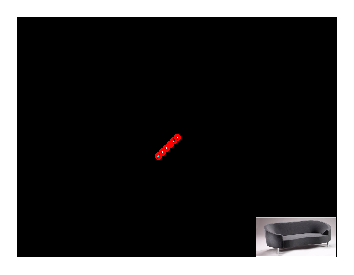
\includegraphics[width=0.5\linewidth]{fig/mass1d-collision1}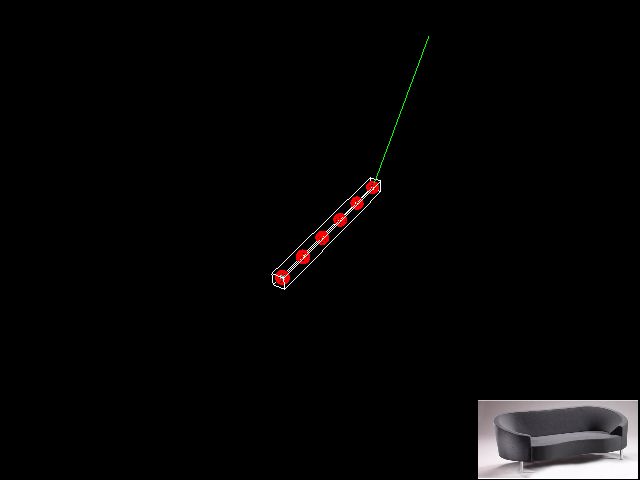
\includegraphics[width=0.5\linewidth]{fig/mass1d-collision2}
\caption{Collisions with 1D particles used to interact with the mouse.}\label{fig:mass1d-collision}
\end{figure}

\begin{figure}
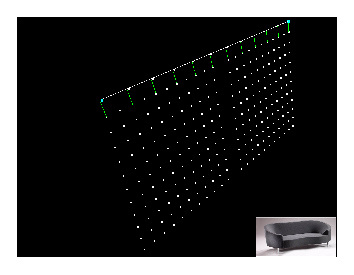
\includegraphics[width=0.5\linewidth]{fig/mass1d-curtain1}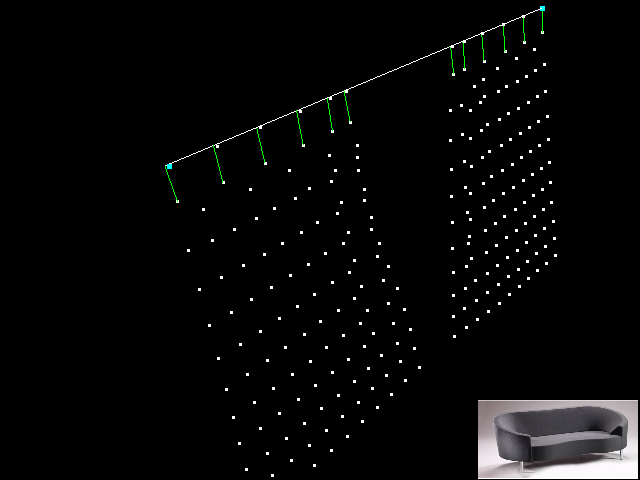
\includegraphics[width=0.5\linewidth]{fig/mass1d-curtain2}\\
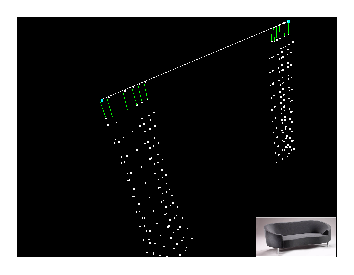
\includegraphics[width=0.5\linewidth]{fig/mass1d-curtain3}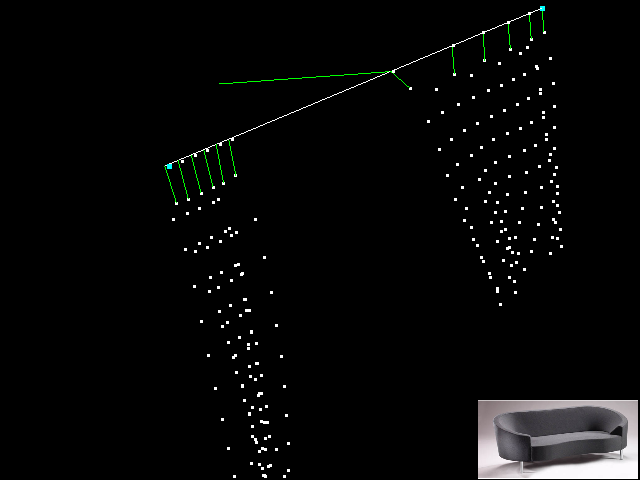
\includegraphics[width=0.5\linewidth]{fig/mass1d-curtain4}%
\caption{1D and 3D particles linked by springs to simulate curtains.}\label{fig:mass1d-curtain}
\end{figure}

You can now pick the particles with the mouse by pressing the shift key and left mouse button, as seen in figure~\ref{fig:mass1d-collision}.

The main advantage of our mapping is that we can combine 1D and 3D particles in the same simulation with forces such as springs applied between them. This is demonstrated in the \texttt{test4.scn} scene, as seen in figure~\ref{fig:mass1d-curtain}.

\section{Non-Linear Mapping}

Mappings are not limited to linear computations. Non-linear mappings can be computed exactly in the apply method, and a local linear approximation can be used for the applyJ and applyJT methods.

For instance, our 1D particles can be mapped to a circle instead of a line. The code for this mapping is available in the
\textcode{Sofa/doc/src\_examples/example3/CircleMapping.cpp} file. It uses the following computations :

\begin{description}
\item[apply] $ \ve x_{out} = \ve{p_0} + \ve{r_x} cos( \ve x_{in} ) + \ve{r_y} sin( \ve x_{in} ) $
\item[applyJ] $ \ve v_{out} = \frac{\delta \ve x_{out}}{\delta \ve x_{in}} \ve v_{in} = ( - \ve{r_x} sin ( \ve x_{in} ) + \ve{r_y} cos ( \ve x_{in} ) ) \ve v_{in} $
\item[applyJT] $ \ve f_{in} = \frac{\delta \ve x_{out}}{\delta \ve x_{in}} \ve f_{out} $ and $ \frac{\delta \ve f_{in}}{\delta \ve x_{in}} = \frac{\delta \ve x_{out}}{\delta \ve x_{in}^2} \ve f_{out} + \frac{\delta \ve x_{out}}{\delta \ve x_{in}} \frac{\delta \ve f_{out}}{\delta \ve x_{out}} $
\end{description}

Note that if we use a local linear approximation, $ \frac{\delta \ve x_{out}}{\delta \ve x_{in}^2} = 0 $ so applyJT is the same for f and df.

\begin{code_cpp}
class CircleMapping : public Sofa::Core::MechanicalMapping< Sofa::Core::MechanicalObject<Vec1dTypes>, Sofa::Core::MechanicalObject<Vec3dTypes> >
{
public:
  // Simplified notation for all involved classes
  typedef Sofa::Core::MechanicalMapping< Sofa::Core::MechanicalObject<Vec1dTypes>, Sofa::Core::MechanicalObject<Vec3dTypes> > BaseMapping;
  typedef BaseMapping::In In;
  typedef BaseMapping::Out Out;
  typedef Out::VecCoord VecCoord;
  typedef Out::VecDeriv VecDeriv;
  typedef Out::Coord Coord;
  typedef Out::Deriv Deriv;

  Coord p0; ///< Origin of the circle
  Deriv rx, ry; ///< Radius of the circle
  
  std::vector<Deriv> dx;
  
  CircleMapping(In* from, Out* to, const std::string& /*name*/)
  : BaseMapping(from, to), p0(0,0,0), rx(1,0,0), ry(0,0,1)
  {
  }
  
  void apply( Out::VecCoord& out, const In::VecCoord& in )
  {
    out.resize(in.size());
    dx.resize(in.size());
    for(unsigned int i=0;i<out.size();i++)
    {
	  double c = cos(in[i]);
	  double s = sin(in[i]);
      out[i] = p0+rx*c+ry*s;
	  dx[i] = rx*(-s)+ry*c;
    }
  }
  
  void applyJ( Out::VecDeriv& out, const In::VecDeriv& in )
  {
    out.resize(in.size());
    for(unsigned int i=0;i<out.size();i++)
      out[i] = dx[i]*in[i];
  }
  
  void applyJT( In::VecDeriv& out, const Out::VecDeriv& in )
  {
    for(unsigned int i=0;i<out.size();i++)
      out[i] += dx[i]*in[i];
  }
};
\end{code_cpp}

To run it, go to \textcode{Sofa/doc/src\_examples/example3} and execute
\begin{code_bash}
./run test5.scn
\end{code_bash}

The result is visible in figure~\ref{fig:mass1d-circle}.

\begin{figure}
\centering
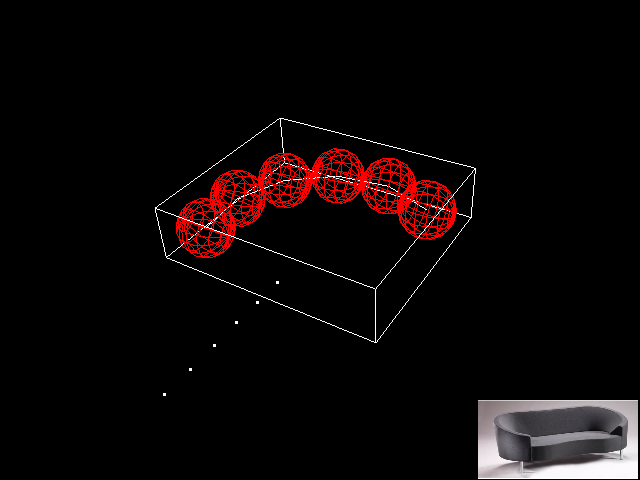
\includegraphics[width=0.5\linewidth]{fig/mass1d-circle1}
\caption{1D particles mapped to a circle.}\label{fig:mass1d-circle}
\end{figure}

\section{Adding a new ForceField}

A ForceField is used to apply forces to mechanical objects in the scene. Its basic role is to compute a force vector $\ve f$ associated with a set of DOFs, given their position $\ve x$ and velocity $\ve v$. To support implicit integration schemes, it must also compute the force derivative $\ve{df}$ given a displacement $\ve {dx}$.

Adding a new ForceField in \sofa{} requires the following steps:

\begin{enumerate}
\item Create the ForceField derived class.
\item Create a method to create an instance of the force field given an XML node.
\item Register the new force field in the \textcode{Sofa::Components::XML::ForceFieldNode::Factory} factory.
\item Create a XML scene file containing a ForceField with the \textit{type} of our class.
\item Have even more fun!
\end{enumerate}

We will now detail these steps implementing \textit{Lennard-Jones} fluid forces. It is a simple force field adding a force between any pair of particles based on a potential related to their distance $d$:\\
$potential = \dfrac{a}{d^\alpha} - \dfrac{b}{d^\beta}$\\
$f = - grad(potential) = ( a \alpha d^{-\alpha-1} - b \beta d^{-\beta-1} ) \ve u$\\
where $\ve u$ is the unit vector between the two particles. This force field has the property to force particles to stay within a certain distance of each other, and is negligible for particles far away from each other, allowing to use a cutoff distance.

Computing the Lennard-Jones forces requires $5$ parameters: $a$, $b$, $\alpha$, $\beta$, and the cutoff distance $d_{max}$. As they are not all meaningful, we will instead allow the user to specify the prefered distance $d_0$ where $f = 0$, as well as the potential value $p_0$ at this point, which controls the force magnitude. The cutoff distance $d_{max}$ will be initialized as $2 d_0$ by default, and we will use $\alpha=6$ and $\beta=12$. The $a$ and $b$ parameters can then be computed as follow:\\
$$
\left\{\begin{array}{rl}
a \alpha d_0^{-\alpha-1} - b \beta d_0^{-\beta-1} &= 0 \\
a d_0^{-\alpha} - b d_0^{-\beta} &= p_0 \\
\end{array}\right\}
\Longrightarrow
\left\{\begin{array}{rl}
b &= a \frac{\alpha}{\beta} d_0^{\beta-\alpha} \\
a d_0^{-\alpha} - a \frac{\alpha}{\beta} d_0^{-\alpha} &= p_0 \\
\end{array}\right\}
\Longrightarrow
\left\{\begin{array}{rl}
a &= \dfrac{p_0 d_0^\alpha}{1 - \frac{\alpha}{\beta}} \\
b &= \dfrac{p_0 d_0^\beta}{\frac{\beta}{\alpha} - 1} \\
\end{array}\right\}
$$

The code for this force field is available in the
\textcode{Sofa/doc/src\_examples/example4/LennardJonesForceField.\{h,inl,cpp\}} files.

\subsection{ForceField Implementation}

A ForceField is attached to a MechanicalObject in the scene. It is implemented by overloading 2 methods:

\begin{description}
\item[addForce] compute force given the position and velocity in the MechanicalObject
\item[addDForce] compute derived force from the displacement in the MechanicalObject
\end{description}

For small or nearly constant forces, the addDForce method can be ignored. For other cases it uses a linear approximation, as it will be used in the inner loop.

The implementation of a force field is dependant on the type of the DOFs to which it applies. For our example, we will create a templated version for genericity, although a non-templated version could also be used if you prefer.

The class declaration is:

\begin{code_cpp}
template<class DataTypes>
class LennardJonesForceField : public Sofa::Core::ForceField, public Sofa::Abstract::VisualModel
{
public:
	typedef Sofa::Core::ForceField Inherit;
	typedef typename DataTypes::VecCoord VecCoord;
	typedef typename DataTypes::VecDeriv VecDeriv;
	typedef typename DataTypes::Coord Coord;
	typedef typename DataTypes::Deriv Deriv;
	typedef typename Coord::value_type Real;
	
protected:
	Sofa::Core::MechanicalModel<DataTypes>* object;
	
	Real a,b,alpha,beta,dmax,fmax;
	Real d0,p0;

	struct DForce
	{
		unsigned int a,b;
		Real df;
	};
	
	std::vector<DForce> dforces;
	
public:
	LennardJonesForceField(Sofa::Core::MechanicalModel<DataTypes>* object, const std::string& /*name*/="")
	: object(object), a(1), b(1), alpha(6), beta(12), dmax(2), fmax(1), d0(1), p0(1)
	{
	}
	
	void setAlpha(Real v) { alpha = v; }
	void setBeta(Real v) { beta = v; }
	void setFMax(Real v) { fmax = v; }
	void setDMax(Real v) { dmax = v; }
	void setD0(Real v) { d0 = v; }
	void setP0(Real v) { p0 = v; }

	virtual void init();
	
	virtual void addForce();
	
	virtual void addDForce();
	
	// -- VisualModel interface
	void draw();
	void initTextures() { }
	void update() { }
};
\end{code_cpp}

The class implementation is:

\begin{code_cpp}
template<class DataTypes>
void LennardJonesForceField<DataTypes>::init()
{
    a = (p0 * (Real)pow(d0,alpha)) / (1-alpha/beta);
    b = (p0 * (Real)pow(d0,beta)) / (beta/alpha-1);
}

template<class DataTypes>
void LennardJonesForceField<DataTypes>::addForce()
{
	Real dmax2 = dmax*dmax;
	VecDeriv& f1 = *this->object->getF();
	VecCoord& p1 = *this->object->getX();
	this->dforces.clear();
	f1.resize(p1.size());
	for (unsigned int ib=1; ib<p1.size(); ib++)
	{
		const Coord pb = p1[ib];
		for (unsigned int ia=0; ia<ib; ia++)
		{
			const Coord pa = p1[ia];
			const Deriv u = pb-pa;
			const Real d2 = u.norm2();
			if (d2 >= dmax2) continue;
			const Real d = (Real)sqrt(d2);
			const Real fa = a*alpha*(Real)pow(d,-alpha-1);
			const Real fb = b*beta*(Real)pow(d,-beta-1);
			Real forceIntensity = fa - fb;
			//std::cout << ia<<"-"<<ib<<" d="<<d<<" f="<<forceIntensity<<std::endl;
			DForce df;
			df.a = ia;
			df.b = ib;
			if (forceIntensity > fmax)
			{
			    forceIntensity = fmax;
			    df.df = 0;
			}
			else
			{
			    df.df = ((-alpha-1)*fa - (-beta-1)*fb)/(d*d2);
			}
			this->dforces.push_back(df);
			const Deriv force = u*(forceIntensity/d);
			f1[ia]+=force;
			f1[ib]-=force;
		}
	}
}

template<class DataTypes>
void LennardJonesForceField<DataTypes>::addDForce()
{
	VecDeriv& f1  = *this->object->getF();
	VecCoord& p1 = *this->object->getX();
	VecDeriv& dx1 = *this->object->getDx();
	f1.resize(dx1.size());
	for (unsigned int i=0; i<this->dforces.size(); i++)
	{
		const DForce& df = this->dforces[i];
		const unsigned int ia = df.a;
		const unsigned int ib = df.b;
		const Deriv u = p1[ib]-p1[ia];
		const Deriv du = dx1[ib]-dx1[ia];
		const Deriv dforce = u * (df.df * (du*u)); 
		f1[ia] += dforce;
		f1[ib] -= dforce;
	}
}

template<class DataTypes>
void LennardJonesForceField<DataTypes>::draw()
{
	if (!Sofa::Components::Scene::getInstance()->getShowForceFields()) return;
	VecCoord& p1 = *this->object->getX();
	glDisable(GL_LIGHTING);
	glColor4f(0,0,1,1);
	glBegin(GL_LINES);
	for (unsigned int i=0; i<this->dforces.size(); i++)
	{
		const DForce& df = this->dforces[i];
		const unsigned int ia = df.a;
		const unsigned int ib = df.b;
		glVertex3d(p1[ia][0],p1[ia][1],p1[ia][2]);
		glVertex3d(p1[ib][0],p1[ib][1],p1[ib][2]);
	}
	glEnd();
}
\end{code_cpp}

\subsection{Instantiation from XML and Registration in Factory}

This process is identical to the corresponding steps in the DynamicObject and Mapping cases, except that the XML Node to use is XML::ForceFieldNode.

In our example, the additional code required for this step is:
\begin{code_cpp}

namespace Sofa { namespace Components { namespace Common {

template<class DataTypes>
void create(LennardJonesForceField<DataTypes>*& obj, XML::Node<Sofa::Core::ForceField>* arg)
{
  XML::createWithParent< LennardJonesForceField<DataTypes>, MechanicalModel<DataTypes> >(obj, arg);
  if (obj!=NULL)
  {
    if (arg->getAttribute("alpha"))  obj->setAlpha(atof(arg->getAttribute("alpha")));
    if (arg->getAttribute("beta"))  obj->setBeta(atof(arg->getAttribute("beta")));
    if (arg->getAttribute("fmax"))  obj->setFMax(atof(arg->getAttribute("fmax")));
    if (arg->getAttribute("dmax"))  obj->setDMax(atof(arg->getAttribute("dmax")));
    else if (arg->getAttribute("d0"))  obj->setDMax(2*atof(arg->getAttribute("d0")));
    if (arg->getAttribute("d0"))  obj->setD0(atof(arg->getAttribute("d0")));
    if (arg->getAttribute("p0"))  obj->setP0(atof(arg->getAttribute("p0")));
  }
} } } }

SOFA_DECL_CLASS(LennardJonesForceField)

// Each instance of our class must be compiled
template class LennardJonesForceField<Vec3fTypes>;
template class LennardJonesForceField<Vec3dTypes>;

// And registered in the Factory
Creator< XML::ForceFieldNode::Factory, LennardJonesForceField<Vec3fTypes> > LennardJonesForceField3fClass("LennardJones", true);
Creator< XML::ForceFieldNode::Factory, LennardJonesForceField<Vec3dTypes> > LennardJonesForceField3dClass("LennardJones", true);
\end{code_cpp}

As our implementation is templated, the create method is also templated, and several Creator must be used, one for each template instantiation we support.

\subsection{Testing}

This new force field can be used to simulate a very simple fluid by initializing a set of particles and applying the Lennard-Jones forces to them.

\begin{code_xml}
<Scene dt="0.005" showBehaviorModels="1" showCollisionModels="1" showMappings="1" showForceFields="1">
	<Group>
		<Solver type="CGImplicit"/>
		<DynamicModel type="MassObject" name="M1" gravity="0 -10 0" mass="0.5">
		<!-- A topology is used here just to set initial particles positions. It is a bad idea because this object has no real topology, but it works... -->
		<Topology type="RegularGrid" nx="8" ny="6" nz="10" xmin="-9" xmax="5" ymin="-8" ymax="2" zmin="-9" zmax="9" />
		<ForceField type="LennardJones" alpha="8" beta="9" p0="-50" d0="1" dmax="4" fmax="1" />
		<!-- The following force fields handle collisions with walls and an inclined floor -->
		<ForceField type="PlaneForceField" normal="1 0 0" d="-10"/>
		<ForceField type="PlaneForceField" normal="-1 0 0" d="-10"/>
		<ForceField type="PlaneForceField" normal="0.1 1 0" d="-10"/>
		<ForceField type="PlaneForceField" normal="0 0 1" d="-10"/>
		<ForceField type="PlaneForceField" normal="0 0 -1" d="-10"/>
		</DynamicModel>
	</Group>
</Scene>
\end{code_xml}

To run it, go to \textcode{Sofa/doc/src\_examples/example4} and execute
\begin{code_bash}
./run test1.scn
\end{code_bash}

\begin{figure}
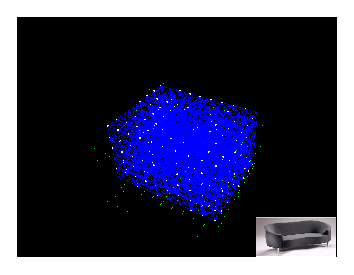
\includegraphics[width=0.33\linewidth]{fig/fluid1-00}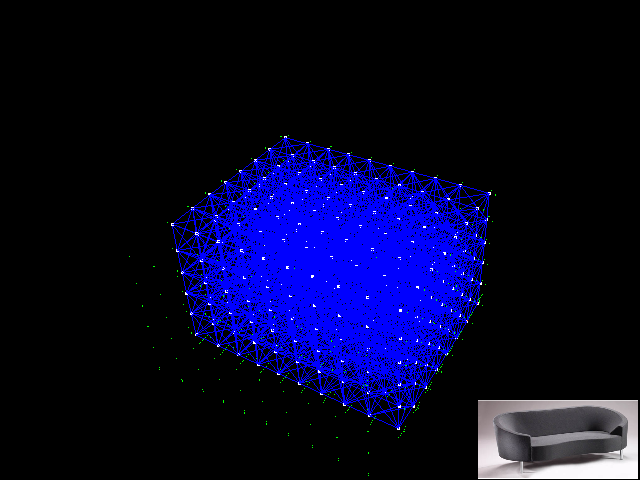
\includegraphics[width=0.33\linewidth]{fig/fluid1-01}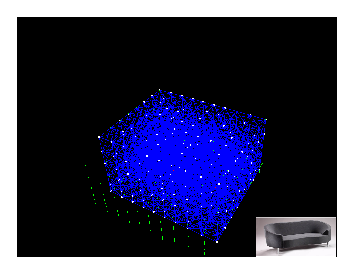
\includegraphics[width=0.33\linewidth]{fig/fluid1-02}\\
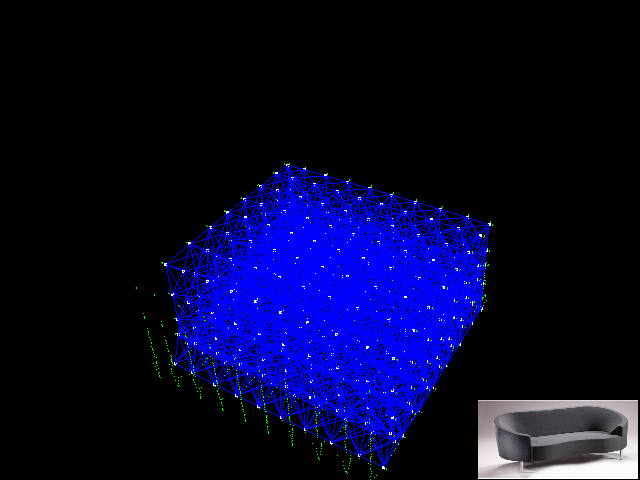
\includegraphics[width=0.33\linewidth]{fig/fluid1-03}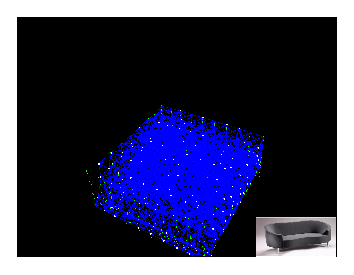
\includegraphics[width=0.33\linewidth]{fig/fluid1-04}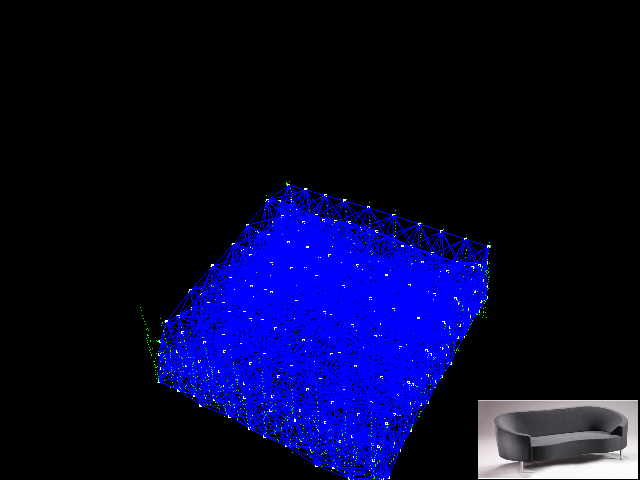
\includegraphics[width=0.33\linewidth]{fig/fluid1-05}\\
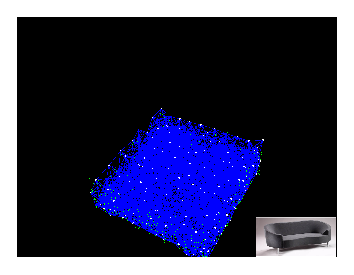
\includegraphics[width=0.33\linewidth]{fig/fluid1-06}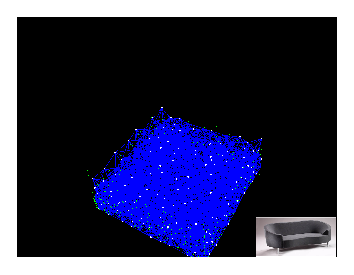
\includegraphics[width=0.33\linewidth]{fig/fluid1-07}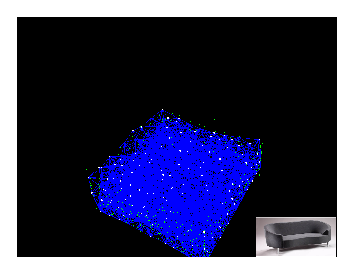
\includegraphics[width=0.33\linewidth]{fig/fluid1-08}\\
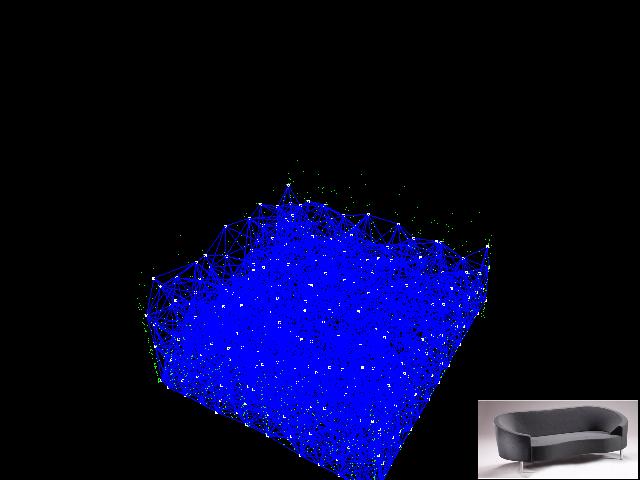
\includegraphics[width=0.33\linewidth]{fig/fluid1-09}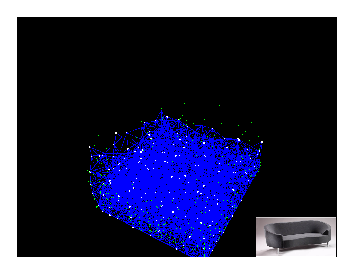
\includegraphics[width=0.33\linewidth]{fig/fluid1-10}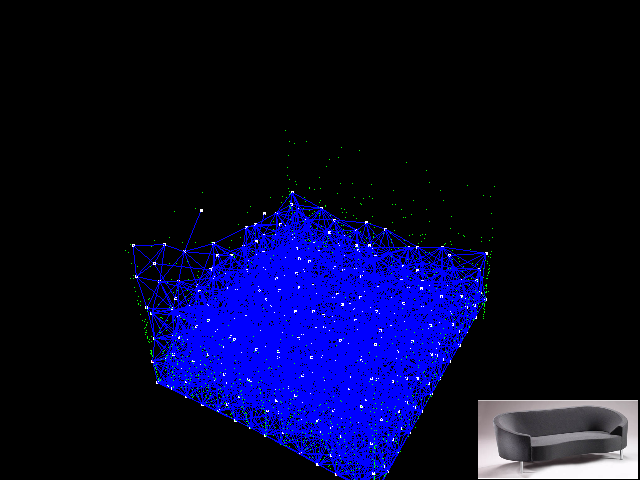
\includegraphics[width=0.33\linewidth]{fig/fluid1-11}
\caption{Fluid animation.}\label{fig:fluid1}
\end{figure}

The resulting animation is shown in figure~\ref{fig:fluid1}.
